\section{Phase transition}

In our leading-order analysis, we saw that $\alpha$ was zero for $\mu_I \leq \bar m$, before it starts to increase for $\mu_I>\bar m$, and that $\bar m = m_\pi$.
The behavior of $\alpha$ is illustrated in \autoref{fig:alpha}.
This is the hallmark of a phase transition, where $\alpha$ is the order parameter.
The behavior of systems near points of phase transition is described by Landau theory~\cite{Peskin:IntroQFT}.
Using \cref{leading order contribution free energy}, we can expand the leading-order free energy in $\alpha$,
\begin{align}
    \nonumber
    \Ef
    & = -f^2 \bar m^2 + f^2 \frac{1}{2}(\bar m^2 - \mu_I^2)\alpha^2
    - \frac{1}{24} f^2 (\bar m^2 - 4 \mu_I^2) \alpha^4 + \Oh[5]{\alpha} \\
    & = \Ef(\alpha=0) + a(\mu_I)\alpha^2 + \frac{1}{2} b(\mu_I)\alpha^4 + \Oh[5]{\alpha},
\end{align}
Notice that near $\mu_I = \bar m$, $b > 0$.
As earlier, the equation that governs $\alpha$ is
\begin{equation}
    \label{landau ginsburg lo}
    \diffp{\Ef}{\alpha} = 2 [a(\mu_I) + b(\mu_I) \alpha^2] \alpha = 0.
\end{equation}
If $a>0$, then $\alpha = 0$ will be the only solution, which gives us the criterion for a phase transition 
\begin{equation}
    a(\mu_I) = 0.
\end{equation}
As expected, this criterion is fulfilled at $\mu_I = \bar m$.
Near $\mu_I = \bar m$, we can write
\begin{equation}
    a = - a_0 (\mu_I - \bar m), \quad b = b_0,
\end{equation}
where $a_0$ and $b_0$ are positive constants, so the solution to \cref{landau ginsburg lo} for $\mu_I>\bar m$ is
\begin{equation}
    \alpha(\mu_I) = \sqrt{\frac{a_0}{b_0}} (\mu_I - \bar m)^{1/2}.
\end{equation}
The free energy around the phase transition is illustrated in \autoref{fig:phase transition}.
\begin{figure}[h]
    \centering
    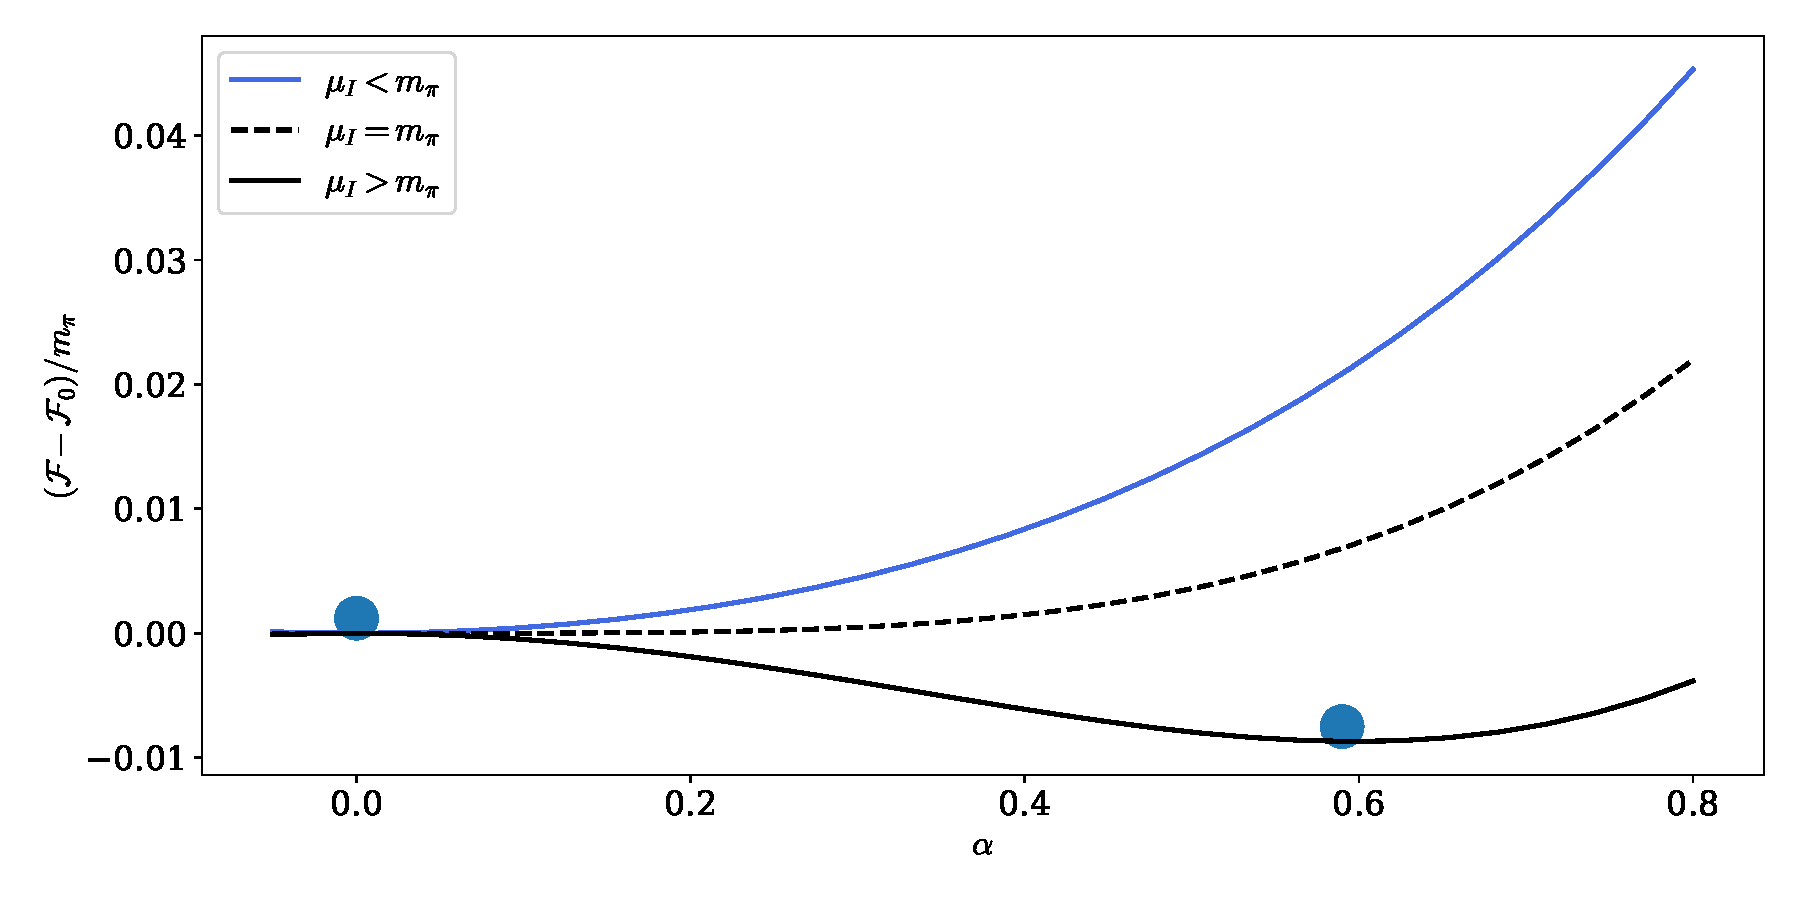
\includegraphics[width=0.9\textwidth]{figurer/numerics/phase_transition.pdf}
    \caption{The plot shows normalized free energy density as a function of $\alpha$, in the two different phases. Each line is a constant $\mu_I$ slice of the surface in \autoref{fig:free energy surface}.}
    \label{fig:phase transition}
\end{figure}

The order parameter $\alpha$ changes continuously as the system undergoes phase-transition.
This means we have a \emph{second order} phase transition.
The power law behavior, $\alpha \propto (\mu_I - \mu_I^c)^\beta$, is typical of systems near a phase transition.
The exponent $\beta$, which in this case equal $1/2$, is called a \emph{critical exponent}.
If we have a system where $b < 0$ near $\mu_I = \bar m$, then we must expand $\Ef$ further to show if the phase transition is continuous or not.
\autoref{fig:free energy surface 2} shows the free energy surface, but modified so that $b_0 < 0$, together with the corresponding value of $\alpha$, which now changes discontinuously at the point of phase transition.
\begin{figure}[h]
    \centering
    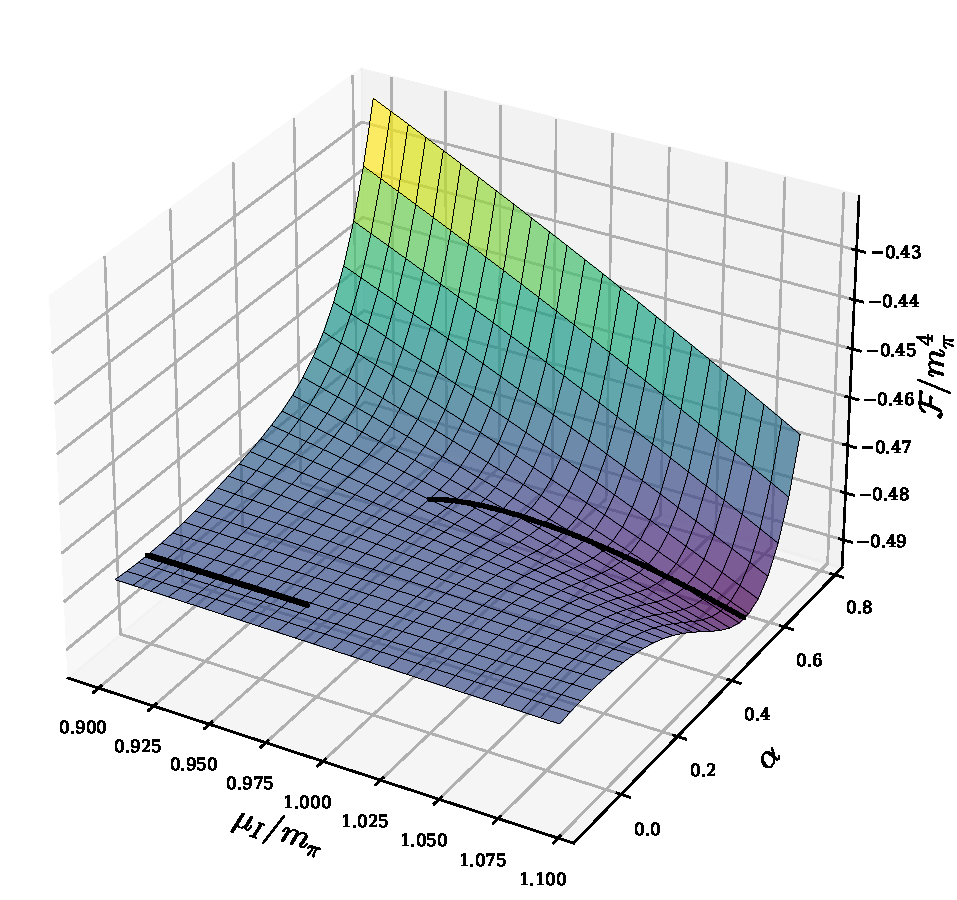
\includegraphics[width=0.7\textwidth]{figurer/numerics/free_energy_surface2.pdf}
    \caption{The surfaceis free energy density, only modified so that $b_0<0$. The black line traces out the minimum for each value of $\mu_I$, which jumps discontinuously at the point of phase transition.}
    \label{fig:free energy surface 2}
\end{figure}


In the vacuum phase, $\alpha = 0$, the ground state is given by 
\begin{equation}
    \Sigma(\pi = 0) = \Sigma_0 = \one,
\end{equation}
where we have used \cref{sigma}.
Under $H = SU(2)_V$, $\Sigma$ transforms as
\begin{equation}
    \Sigma(x) \rightarrow \Sigma'(x) = V \Sigma(x) V^\dagger,
    \quad
    V = \exp{i \frac{1}{2} \theta_a \tau_a},
\end{equation}
We see that the vacuum phase ground state is invariant under $H$.
However, for $\alpha \neq 0$, the ground state is shifted to
\begin{equation}
    \Sigma(\pi=0) = A_\alpha \Sigma_0 A_\alpha = \exp{i \alpha \tau_1}.
\end{equation}
This is not, in general, invariant under transformations in $H$, and generators $\tau_2$ and $\tau_3$ are broken.
The new ground state corresponds to a condensate of the $\pi_1$-particle, as it is defined in the vacuum state.
In \autoref{fig:masses}, we saw that the mass of the $m_-$ particle vanishes, so we identify this particle with the corresponding Goldstone mode.
There is only one Goldstone mode, however this is not a Lorentz invariant system, in which case we cannot guarantee one massless mode per broken generator.

To find the value of $\mu_I$ to next-to-leading order, we must expand the NLO free energy in powers of $\alpha$
When we expand the static, second order Lagrangian to $\alpha^2$, we get
\begin{align}
    \Ef_4^{(0)}
    &= - (l_3 + l_4)\bar m^4 + [(l_3 + l_4)\bar m^4 -l_4 \bar m^2\mu_I^2]\alpha^2
    \\
    & =
    \const + 
    \frac{\mu^{-2\epsilon}}{(4\pi)^2}
    \left[
        \left(
            \bar l_4 - \frac{1}{4}\bar l_3
        \right)\bar m^4
        -\bar l_4\bar m^2\mu_I^2
        -\left(
            1 + \frac{1}{\epsilon} + \ln\frac{\tilde \mu^2}{M^2}
        \right)
        \left(\frac{3}{4}\bar m^2 - \mu_I^2\right)\bar m^2
    \right]\alpha^2,
\end{align}
where $\const$ is independent of $\alpha$, and thus not of interest.
From the one-loop correction, we have the contributions
\begin{equation}
    \Ef_2^{(1)} = i \frac{1}{2}\int \frac{\dd^4 p}{(2\pi)^2} \ln(-p^2 + m_3^2)
    +  i \frac{1}{2} \int \frac{\dd^4 p}{(2\pi)^2} \ln[(-p^2 + m_1^2)(-p^2 + m_2^2) - p_0^2 m_{12}^2].
\end{equation}
The first integral is the same free energy contribution from the $\pi_0$-particle as we have calculated earlier in \cref{Free energy pi 0}, and it reads
\begin{equation}
    \Ef_{\pi_0}^{(1)}
    = i \frac{1}{2}\int \frac{\dd^4 p}{(2\pi)^2} \ln(-p^2 + m_3^2)
    = - \mu^{-2\epsilon}\frac{1}{4} \frac{m_3^4}{(4 \pi)^2}
    \left(\frac{1}{\epsilon} + \frac{3}{2} + \ln \frac{\tilde \mu^2}{m_3^2}\right).
\end{equation}
The mass $m_3$ is dependent on $\alpha$, and has the expansion
\begin{align*}
    m_3^4
    &= \bar m^4 + \bar m^2(2\mu_I^2 - \bar m^2)\alpha^2+ \Oh[4]{\alpha}, \\
    \ln \frac{\mu^2}{m_3^2}
    &=
    \ln \frac{\mu^2}{\bar m_3^2} - \frac{1}{2} \frac{(2\mu_I^2 - \bar m^2)}{\bar m^2}+ \Oh[4]{\alpha}.
\end{align*}
In the second integral, we rewrite the argument of the logarithm as
\begin{equation}
    (-p^2 + m_1^2)(-p^2 + m_2^2) - p_0^2 m_{12}^2
    =  \left[-p^2 + \frac{1}{2}(m_1^2 + m_2^2)\right]^2 - p_0^2 m_{12}^2 - \frac{1}{4}(m_1^2 - m_2^2)^2.
\end{equation}
When we calculate the $\alpha$ dependence of the last term, we get  $(m_1^2 - m_2^2)^2 = \mu^4 \sin^4\alpha = \Oh[4]{\alpha}$, which means that for our purposes, we can ignore this term.
We further rewrite the remaining expression by factoring it,
\begin{equation}
    \left[-p^2 + \frac{1}{2}(m_1^2 + m_2^2)\right]^2 - p_0^2 m_{12}^2
    = \left[-p^2 + \frac{1}{2}(m_1^2 + m_2^2) - p_0 m_{12} \right]
    \left[-p^2 + \frac{1}{2}(m_1^2 + m_2^2) + p_0 m_{12} \right]
\end{equation}
We then complete the square in each of the factors,
\begin{equation}
    - p^2 + \frac{1}{2}(m_1^2 + m_2^2) \pm p_0 m_{12}
    = - \left(p_0 \mp \frac{1}{2}m_{12}\right)^2 + |\vv p|^2 + m_4^2,
\end{equation}
where
\begin{align}
    m_4^2 &= \frac{1}{2}\left(m_1^2 +m_2^2 +\frac{1}{2}m_{12}\right)
    = \bar m^2 \cos\alpha + \frac{1}{2} \mu_I^2 \sin^2 \alpha, \\
    m_4^4
    &= \bar m^4 - \bar m^2(m^2 + \mu_I^2) \alpha^2 + \Oh[4]{\alpha}, \\
    \ln \frac{\mu^2}{m_4^2} 
    &= \ln \frac{\mu_I^2}{\bar m^2} + \frac{1}{2}\frac{\bar m^2 + \mu_I^2}{\bar m^2}\alpha^2
    + \Oh[4]{\alpha}.
\end{align}
After a shift of variables, the integral has the same form as the logarithmic integrals we have calculated earlier, which gives us the result
\begin{equation}
    \Ef_{\pi_\pm}
    = i \int \frac{\dd^4}{(2\pi)^4}
    \ln(-p^2 + m_4^2)
    = 
    - \mu^{-2\epsilon}\frac{1}{2} \frac{m_4^4}{(4 \pi)^2}
    \left(\frac{1}{\epsilon} + \frac{3}{2} + \ln \frac{\tilde \mu^2}{m_4^2}\right)
\end{equation}
Combining these two contributions to the one-loop correction of the free energy gives
\begin{align*}
    \Ef_2^{(1)}
    &=
    \mathrm{const.}
    +
    \frac{\mu^{-2 \epsilon } }{(4 \pi)^2} 
    \left(1 + \frac{1}{\epsilon} + \ln \frac{\tilde \mu^2}{m^2}\right)
    \left(\frac{3}{4}m^2 - \mu_I^2\right)
    \bar m^2 \alpha^2
\end{align*}
We see that again, the $\epsilon^{-1}$ will cancel when we combine the NLO-terms.
The NLO correction to the free energy becomes
\begin{align}
    \tilde \Ef_1
    & = 
    \const+ 
    \frac{1}{(4\pi)^2}
    \left[
        \left(
            \bar l_4 - \frac{1}{4}\bar l_3
        \right)\bar m^4
        -\bar l_4\bar m^2\mu_I^2
        + \ln\frac{M^2}{\bar m^2}
        \left(\frac{3}{4}\bar m^2 - \mu_I^2\right)\bar m^2
    \right]\alpha^2
    + \Oh[4]{\alpha}.
\end{align}
All coupling constants are measured at $M = m_\pi$.
Using this in the logarithm gives,
\begin{equation}
    \ln \frac{M^2}{\bar m^2}
    = \ln \frac{m_\pi^2}{\bar m^2}
    = \ln \left[1 + \Oh[2]{(\bar m/f)} \right]
    = \Oh[2]{(\bar m/f)}.
\end{equation}
The term proportional to the logarithm thus vanish to next-to-leading order.
Combining these expressions give total NLO free energy, up to second order in $\alpha$, is
\begin{equation}
    \Ef_{\mathrm{NLO}}
    =
    \Ef_{\mathrm{NLO}}(\alpha = 0)
    +
    \frac{1}{2} f^2 \bar m^2
    \left(
        1
        -
        \frac{1}{2}
        \frac{\bar l_3 - 4 \bar l_4}{(4 \pi)^2} \frac{\bar m^2}{f^2}
    \right)\alpha^2
    - \frac{1}{2}f^2 \mu_I^2
    \left(
        1
        +
        \frac{2 \bar l_4}{(4 \pi)^2}
        \frac{\bar m^2}{f^2}
    \right) \alpha^2
    + \Oh[4]{\alpha}.
\end{equation}
We now insert the physical constants $f_\pi$ and $m_\pi$, by using the next-to-leading order expressions \cref{equation bare mass} and \cref{equation bare decay constant}.
First, notice that
\begin{equation}
    f_\pi^2 m_\pi^2
    = f^2 \bar m^2
    \left[
        1 - \frac{1}{2} \frac{\bar l_3 - 4 \bar l_4}{(4 \pi)^2} \frac{\bar m^2}{f^2}
        +
        \Oh[]{\frac{\bar m^4}{f^4}}
    \right],
\end{equation}
which means that the NLO free energy has the same structure as the leading order expression,
\begin{equation}
    \Ef_{\mathrm{NLO}}
    =
    \Ef_{\mathrm{NLO}}(\alpha = 0)
    + \frac{1}{2}f_\pi^2 (m_\pi^2 - \mu_I^2 )\alpha^2
    + \Oh[4]{\alpha}.
\end{equation}
This shows that the critical isospin chemical potential is $\mu_I^c = m_\pi$, also at next-to-leading order.
We expect this to hold to all orders in perturbation theory.
